\section{Test runs}
	Testing is an essential aspect while developing a product. During development of the protocol several tests were run and the successful ones reaching certain milestones will be described. This also gives more insight in the complete development cycle and what the current state of the protocol is. Xilinx Vivado 2016.4 has been used during development.
	
	\subsection{Early testing}
	At the 12th of June 2018 the first design had been implemented and tested on hardware. The core worked, but several bugs appeared and the interface didn't completely behave as intended. Some packets were lost in the transmission and their placeholder were filled with packets that appeared at the position before them. Many duplicates could be seen. Further investigation quickly resulted in the conclusion the framing and deframing of bursts didn't operate flawlessly. However the positive news was that the other components did behave as expected.
	
	After exhaustive debugging and testing of the framing and deframing of bursts, another test run followed at June the 18th. This time the core behaved as expected and this was the first successful test of Core1990!
	
	\begin{figure}[H]
		\centering
		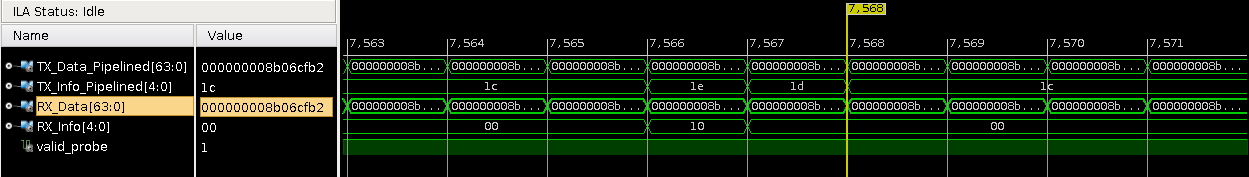
\includegraphics[width=\textwidth]{Test_Hardware_1.png}	
		\caption{The ILA during test.}
		\label{Fig:Test_Hardware_1}
	\end{figure}
	
	In Figure \ref{Fig:Test_Hardware_1} a small fragment of the analyzed data is visualized. The TX data is pipelined to compensate the duration it takes to get data from the TX input to the RX output. To be exact this was 25 clock cycles. The TX and RX data are exact the same, which indicates the data has been transmitted over fiber and was received without any corruption. The valid probing signal also confirms this.
	Additionally the info signals stand for the EOP, SOP and valid bytes. Here some improvements are still to be made but the most important part is the data itself arriving flawlessly.
	
%	\begin{figure}[H]
%		\centering
%		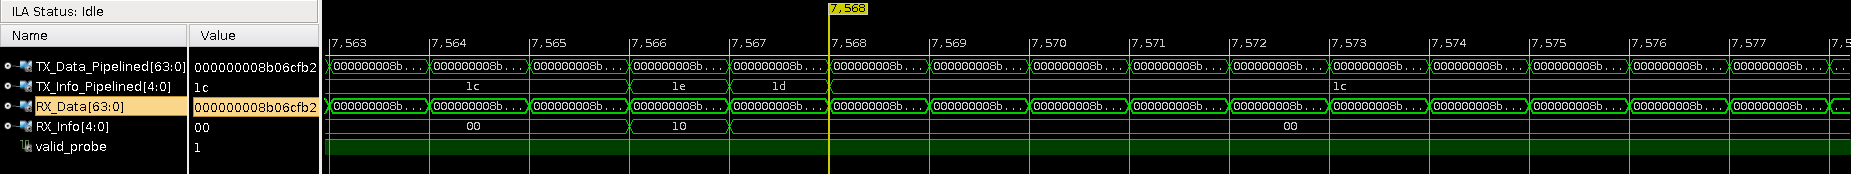
\includegraphics[width=\textwidth]{Test_Hardware_2.png}	
%		\caption{Overview of the decoder block.}
%		\label{Fig:Test_Hardware_2}
%	\end{figure}
	
	\begin{figure}[H]
		\centering
		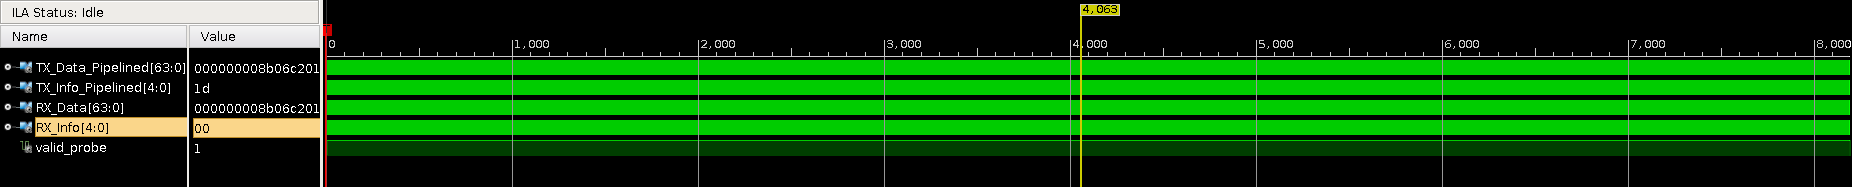
\includegraphics[width=\textwidth]{Test_Hardware_3.png}	
		\caption{The full sample range of the ILA during test.}
		\label{Fig:Test_Hardware_3}
	\end{figure}
	
	Figure \ref{Fig:Test_Hardware_3} shows another run showing the full 8192 samples the ILA could take. During this time the valid probing signal never contains a falling edge which indicates no errors in the data integrity did appear.
	The test has been performed with the data itself being generated at 40 MHz so this means the data rate itself was 2,560 Gbps but the core was still functioning at 156,25 MHz which means the lane rate still performed at its nominal 10 Gbps bandwidth. The core waits for data and now about every four cycles one new packet was ready. Further testing can be done at higher rates.
	
	In short this test contained burst framing/deframing, meta framing/deframing, scrambling/descrambling and encoding/decoding which all performed flawlessly under test.
	Generating CRC and checking was also included but not analyzed using the ILA so this still has to be proven. At this point flow control is still in early stage so this doesn't count in this test.
	
	\subsection{Clock troubleshooting}
	Earlier test introduced a strange problem while communicating between two boards. Both links were in lock for a while but suddenly after a undefined period of time lost lock while this didn't happen with the loop-back tests. This clearly indicated clocking signals between the boards weren't correctly synchronized and started to mismatch.
	
	The problem was fixed by changing the transceiver clock (GTREFCLK) from the 125 MHz SGMIICLK to a 156,25 MHz reference clock. This was generated by the on-board Si570 clock generator IC. On of the downsides was that the Si570 output was not directly connected to one of the clock inputs of the transceiver but a different IO on the FPGA. However one of the reference clock inputs of the transceiver is physically connected to on-board SMA connectors, this can be used to provide the 156,25 MHz input.
	
	To solve the clock problem, the Si570 differential signal entered the FPGA and was converted to single-ended with an IBUFDS. After this the signal was converted to a differential output with an OBUFDS. This way the clock signal has been routed to IO that has been connected to SMA connectors. An external connection can now be made from the output 156,25 MHz signal to the transceiver inputs. Figure \ref{Fig:VC707_SMA} shows a picture of the VC707 board using the Si570 generated clock for the transceiver.
	
	\begin{figure}[H]
		\centering
		\includegraphics[width=0.95\textwidth]{VC707_SMA.jpg}	
		\caption{Using the Si570 clock on the VC707.}
		\label{Fig:VC707_SMA}
	\end{figure}

	Schematically this looks like depicted in Figure \ref{Fig:VC707_Clock_Schematic} which shows the connection between the Si570 and external transceiver clock input. All signals have been named according to the original VC707 schematic by Xilinx \cite{VC707_Schematic}.
	
	\begin{figure}[H]
		\centering
		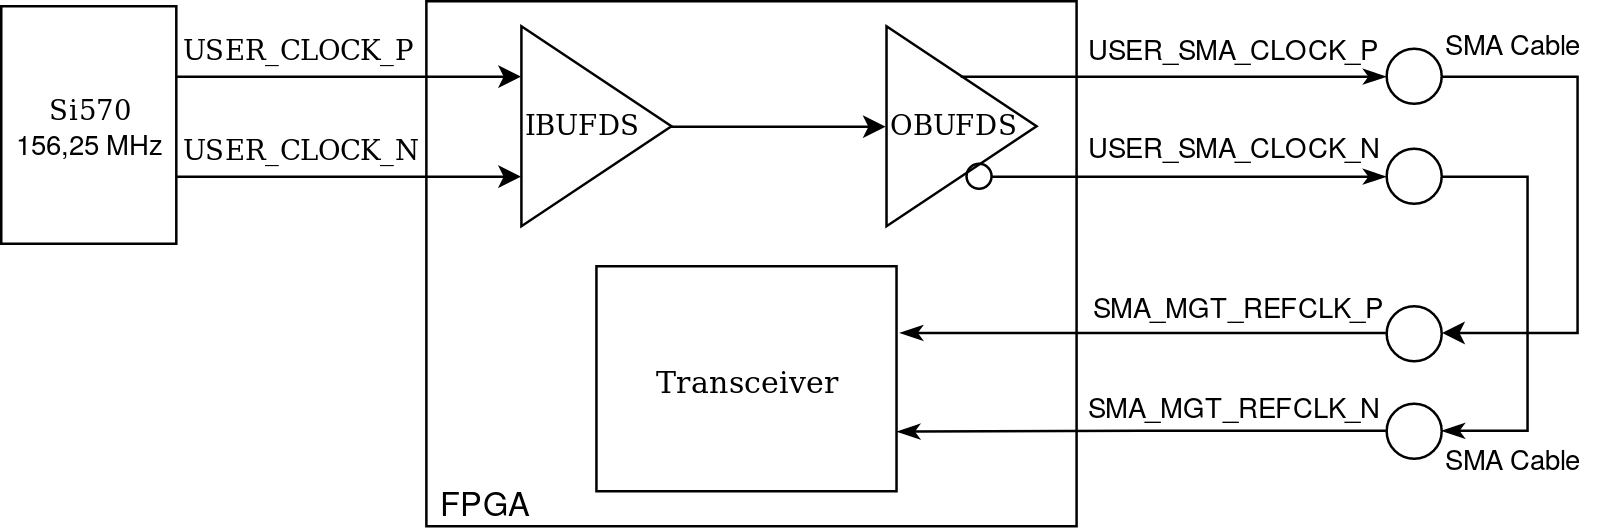
\includegraphics[width=\textwidth]{VC707_Clock_Schematic.png}	
		\caption{Schematically viewed configuration of the Si570 clock on the VC707.}
		\label{Fig:VC707_Clock_Schematic}
	\end{figure}

	\subsection{Communication between boards}
	Another run at the 27th of June proved better results. Instead of a single board with a loop-back fiber, now two VC707 board could be used. Because of the newly connected 156,25 MHz reference clock, the link was stable and didn't lose lock. Figure \ref{Fig:VC707_Multi_Board} shows the two connected boards. Even unplugging the fiber cable and reconnecting it caused an immediate lock which indicates the link had a self recovering capability.
	
	\begin{figure}[H]
		\centering
		\includegraphics[width=\textwidth]{VC707_Multi_Board.jpg}	
		\caption{Testing communication between two VC707 boards.}
		\label{Fig:VC707_Multi_Board}
	\end{figure}
	
	Both boards have a status led that indicated lock of the decoder and descrambler which was always on. A good indication but to be completely sure the lock was very stable, the ILA was used to get a better view.
	
	\begin{figure}[H]
		\centering
		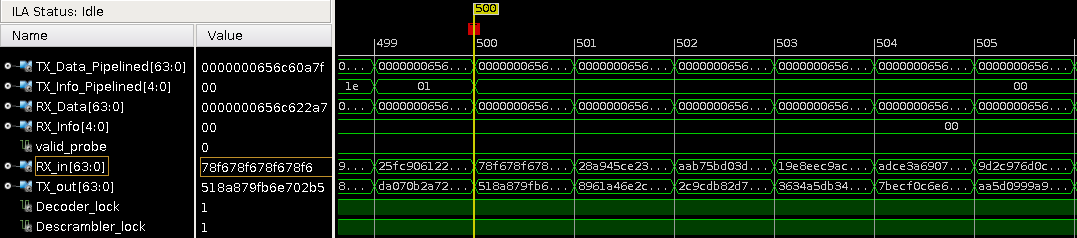
\includegraphics[width=\textwidth]{VC707_Multi_Board_Waveform.png}	
		\caption{Wave forms captured during the communication between VC707 boards.}
		\label{Fig:VC707_Multi_Board_Waveform}
	\end{figure}
	 
	A small piece of data viewed with the ILA can been seen in Figure \ref{Fig:VC707_Multi_Board_Waveform}. At the yellow marker line a synchronization word being received and followed by the scrambler state can be seen. The data differs a bit but that is because the boards differ some cycles from each other and the longer fiber wire used causes some extra clock cycles delay. 
	
	In this case the data generator was connected to a clock of 150 MHz which means the line transferred an amount of 9,6 Gbps on user data. However sometimes the TX FIFO became a bit full and the data generator had to wait. It should also be taken into account the overhead plays a role and 9,6 Gbps plus this overhead could easily require more than the 10 Gbps transfer speed of the transceiver. 
	
	While it was not easy to verify, the inspected data by hand was correct and didn't show the data missing. However not everything could be checked by far and this process should be automated for the next run. In case error's appear these will be easier to detect.
	\vspace{\baselineskip} \newline
	For testing this example design with the two boards connected, several thing mentioned underneath were required.
	\begin{itemize}
		\item Two VC707 boards (Including power supply and USB cable)
		\item Four SMA-SMA (female-female) cables
		\item Two fiber wires
		\item Two SFP+ optical - electrical modules
	\end{itemize}
	
\newpage
